\documentclass[aspectratio=169]{beamer}
\mode<presentation>

\usepackage{default}
\usepackage{multimedia}
\usepackage{multicol}
\usepackage[export]{adjustbox}

\usetheme{default}
\beamertemplatenavigationsymbolsempty

\title{AutoRally}
\subtitle{Scale Autonomous Racing at Georgia Tech}
\author{Matthew Barulic}
\date{\today}
\institute{}

\begin{document}
	
\begin{frame}
\titlepage
\hypertarget{titlePage}{}
\end{frame}

\begin{frame}{Outline}
\tableofcontents
\end{frame}

\section{The Platform}

\begin{frame}{The AutoRally Platform}
\begin{center}
\includegraphics[max size={\linewidth}{0.85\textheight}]{platform_clean.jpg}
\end{center}
\end{frame}

\begin{frame}{The Chassis}
\begin{center}
\includegraphics[max size={\linewidth}{0.85\textheight}]{chassis.jpg}
\end{center}

\end{frame}

\begin{frame}{The Compute Box}
\begin{center}
\includegraphics[max size={\linewidth}{0.85\textheight}]{compute_box.jpg}
\end{center}
\end{frame}

\begin{frame}{The Compute Box}
\begin{center}
\includegraphics[max size={\linewidth}{0.85\textheight}]{compute_box_open.jpg}
\end{center}
\end{frame}

\begin{frame}{The Tracks}
\begin{center}
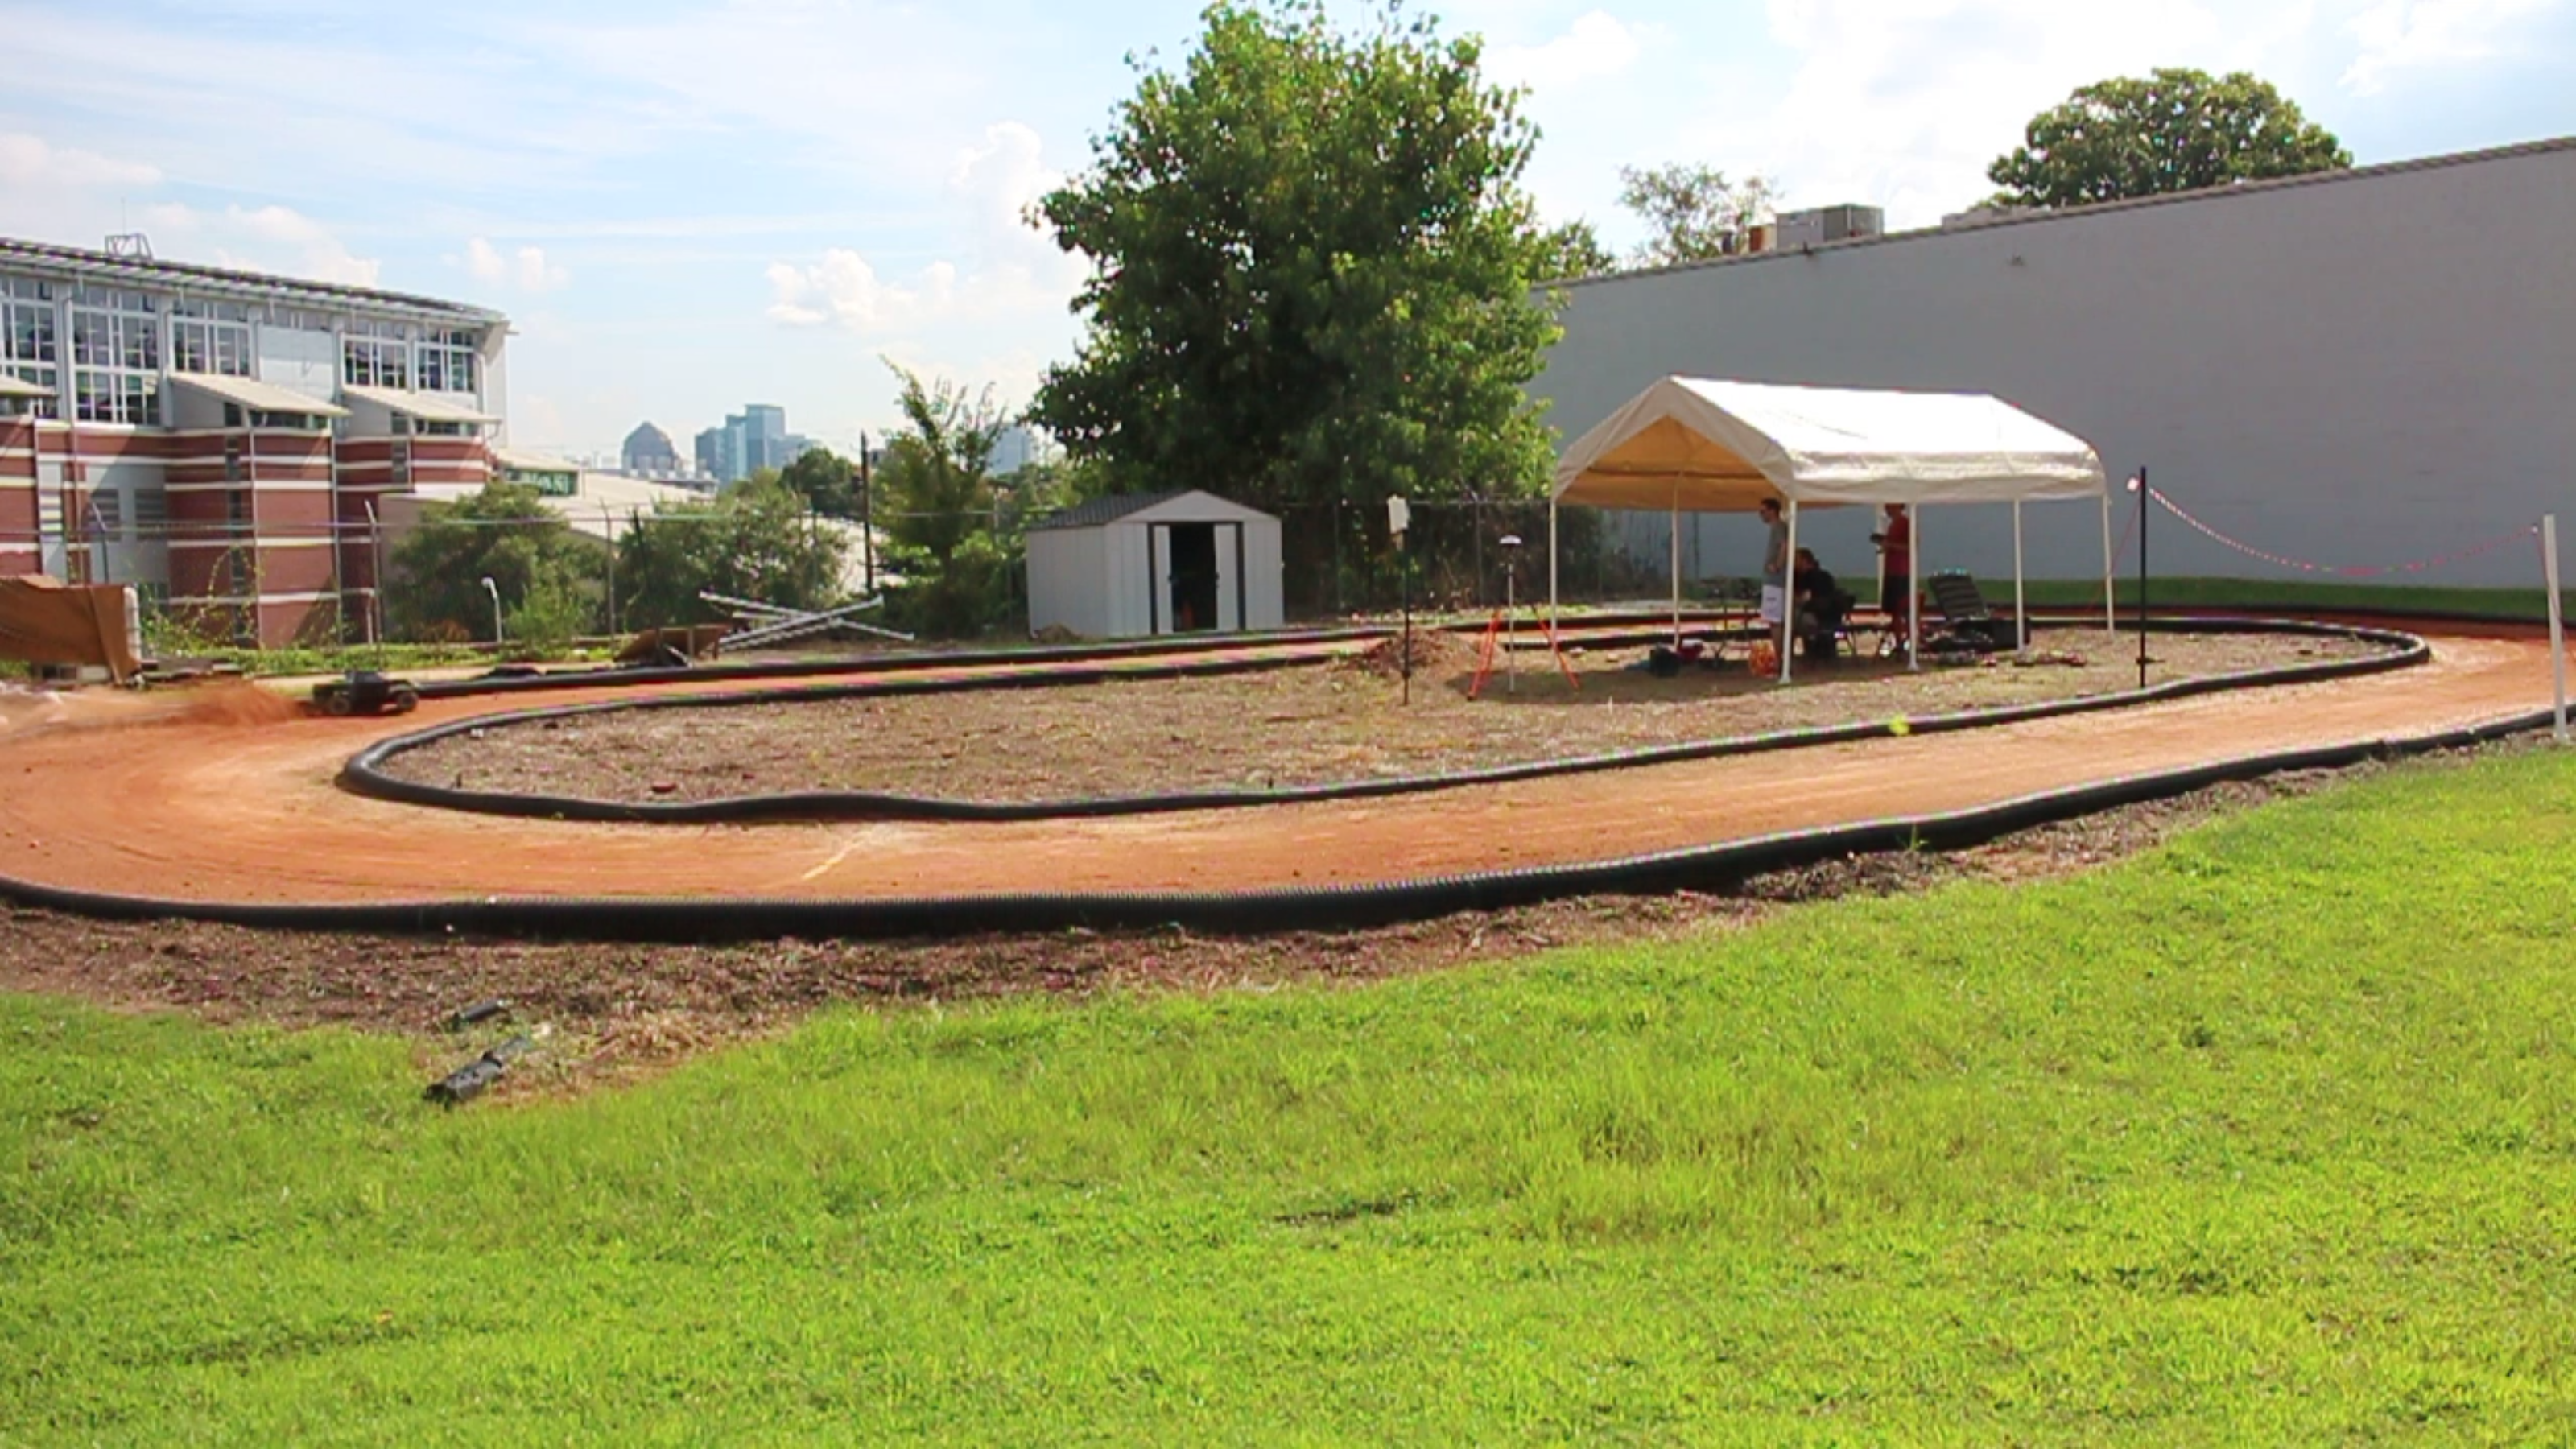
\includegraphics[max size={\linewidth}{0.85\textheight}]{gtarfTrack.png}
\end{center}
\end{frame}

\begin{frame}{The Tracks}
\begin{center}
\includegraphics[max size={\linewidth}{0.85\textheight}]{gtarfTrack2.jpg}
\end{center}
\end{frame}

\begin{frame}{The Challenge}
\movie[autostart,loop]{\includegraphics[max size={\linewidth}{0.85\textheight}]{RSS_2018_Preview.png}}{RSS_2018.mp4}
\end{frame}

\begin{frame}{The Challenge}
\movie[autostart,loop]{\includegraphics[max size={\linewidth}{0.85\textheight}]{Crash_2017_Preview.png}}{Crash_2017.mp4}
\end{frame}

\begin{frame}{The Challenge}
\movie[autostart,loop]{\includegraphics[max size={\linewidth}{0.85\textheight}]{Crash_2018_Preview.png}}{Crash_2018.mp4}
\end{frame}

\section{The Research}

\begin{frame}{Publications Using the AutoRally Platform}
\begin{multicols}{2}
	\fontsize{5pt}{0}\selectfont
	\begin{itemize}
		\item Ensemble Bayesian Decision Making with Redundant Deep Perceptual Control Policies. Keuntaek Lee, Ziyi Wang, Bogdan Vlahov, Harleen Brar, Evangelos A Theodorou. To be appear, ICMLA, 2019.
		\item Perceptual Attention-based Predictive Control. Keuntaek Lee, Gabriel Nakajima An, Viacheslav Zakharov, Evangelos A Theodorou. To be appear, CoRL, 2019.
		\item Locally Weighted Regression Pseudo-Rehearsal for Online Learning of Vehicle Dynamics. Grady Williams, Brian Goldfain, James M Rehg, Evangelos A Theodorou. To be appear, CoRL, 2019.
		\item An Online Learning Approach to Model Predictive Control. Nolan Wagener, Ching-An Cheng, Jacob Sacks, Byron Boots. IEEE Robotics and Automation Letters (RA-L), 2019.
		\item Early Failure Detection of Deep End-to-End Control Policy by Reinforcement Learning. Keuntaek Lee, Kamil Saigol, Evangelos A Theodorou. IEEE International Conference on Robotics and Automation (ICRA), 2019.
		\item Vision-Based High-Speed Driving With a Deep Dynamic Observer. Paul Drews, Grady Williams, Brian Goldfain, Evangelos A Theodorou, James M Rehg. IEEE Robotics and Automation Letters (RA-L), 2019.
		\item Robust Sampling Based Model Predictive Control with Sparse Objective Information. Grady Williams, Brian Goldfain, Paul Drews, Kamil Saigol, James M Rehg, Evangelos Theodorou. Robotics: Science and Systems (RSS), 2018.
		\item Agile autonomous driving using end-to-end deep imitation learning. Yunpeng Pan, Ching-An Cheng, Kamil Saigol, Keuntaek Lee, Xinyan Yan, Evangelos Theodorou, Byron Boots. Robotics: Science and Systems (RSS), 2018.
		\item Best Response Model Predictive Control for Agile Interactions Between Autonomous Ground Vehicles. Grady Williams, Brian Goldfain, Paul Drews, James M Rehg, Evangelos A Theodorou. IEEE International Conference on Robotics and Automation (ICRA), 2018.
		\item Information-Theoretic Model Predictive Control: Theory and Applications to Autonomous Driving. Grady Williams, Paul Drews, Brian Goldfain, James M Rehg, Evangelos A Theodorou. IEEE Transactions on Robotics (T-RO), 2018.
		\item Aggressive Deep Driving: Model Predictive Control with a CNN Cost Model. Paul Drews, Grady Williams, Brian Goldfain, Evangelos A. Theodorou, James M. Rehg. Conference on Robotic Learning (CoRL), 2017.
		\item Information theoretic MPC for model-based reinforcement learning. Grady Williams, Paul Drews, Brian Goldfain, James M Rehg, Evangelos A Theodorou. IEEE International Conference on Robotics and Automation (ICRA), 2017.
		\item Vehicle Modeling and Parameter Estimation Using Adaptive Limited Memory Joint-State UKF. Changxi You, Panagiotis Tsiotras. American Control Conference (ACC), 2017.
		\item Aggressive driving with model predictive path integral control. Grady Williams, Paul Drews, Brian Goldfain, James M Rehg, Evangelos A Theodorou. IEEE International Conference on Robotics and Automation (ICRA), 2016.
	\end{itemize}
\end{multicols}
\end{frame}

\begin{frame}{Publications Using the AutoRally Platform}
\begin{multicols}{2}
	\fontsize{5pt}{0}\selectfont
	\begin{itemize}
		\item Ensemble Bayesian Decision Making with Redundant Deep Perceptual Control Policies. Keuntaek Lee, Ziyi Wang, Bogdan Vlahov, Harleen Brar, Evangelos A Theodorou. To be appear, ICMLA, 2019.
		\item Perceptual Attention-based Predictive Control. Keuntaek Lee, Gabriel Nakajima An, Viacheslav Zakharov, Evangelos A Theodorou. To be appear, CoRL, 2019.
		\item Locally Weighted Regression Pseudo-Rehearsal for Online Learning of Vehicle Dynamics. Grady Williams, Brian Goldfain, James M Rehg, Evangelos A Theodorou. To be appear, CoRL, 2019.
		\item An Online Learning Approach to Model Predictive Control. Nolan Wagener, Ching-An Cheng, Jacob Sacks, Byron Boots. IEEE Robotics and Automation Letters (RA-L), 2019.
		\item Early Failure Detection of Deep End-to-End Control Policy by Reinforcement Learning. Keuntaek Lee, Kamil Saigol, Evangelos A Theodorou. IEEE International Conference on Robotics and Automation (ICRA), 2019.
		\item \alert{Vision-Based High-Speed Driving With a Deep Dynamic Observer. Paul Drews, Grady Williams, Brian Goldfain, Evangelos A Theodorou, James M Rehg. IEEE Robotics and Automation Letters (RA-L), 2019.}
		\item Robust Sampling Based Model Predictive Control with Sparse Objective Information. Grady Williams, Brian Goldfain, Paul Drews, Kamil Saigol, James M Rehg, Evangelos Theodorou. Robotics: Science and Systems (RSS), 2018.
		\item Agile autonomous driving using end-to-end deep imitation learning. Yunpeng Pan, Ching-An Cheng, Kamil Saigol, Keuntaek Lee, Xinyan Yan, Evangelos Theodorou, Byron Boots. Robotics: Science and Systems (RSS), 2018.
		\item Best Response Model Predictive Control for Agile Interactions Between Autonomous Ground Vehicles. Grady Williams, Brian Goldfain, Paul Drews, James M Rehg, Evangelos A Theodorou. IEEE International Conference on Robotics and Automation (ICRA), 2018.
		\item Information-Theoretic Model Predictive Control: Theory and Applications to Autonomous Driving. Grady Williams, Paul Drews, Brian Goldfain, James M Rehg, Evangelos A Theodorou. IEEE Transactions on Robotics (T-RO), 2018.
		\item Aggressive Deep Driving: Model Predictive Control with a CNN Cost Model. Paul Drews, Grady Williams, Brian Goldfain, Evangelos A. Theodorou, James M. Rehg. Conference on Robotic Learning (CoRL), 2017.
		\item Information theoretic MPC for model-based reinforcement learning. Grady Williams, Paul Drews, Brian Goldfain, James M Rehg, Evangelos A Theodorou. IEEE International Conference on Robotics and Automation (ICRA), 2017.
		\item Vehicle Modeling and Parameter Estimation Using Adaptive Limited Memory Joint-State UKF. Changxi You, Panagiotis Tsiotras. American Control Conference (ACC), 2017.
		\item \alert{Aggressive driving with model predictive path integral control. Grady Williams, Paul Drews, Brian Goldfain, James M Rehg, Evangelos A Theodorou. IEEE International Conference on Robotics and Automation (ICRA), 2016.}
	\end{itemize}
\end{multicols}
\end{frame}

\begin{frame}{MPPI}
Model Predictive Path Integral
\movie[autostart,loop]{\includegraphics[max size={\linewidth}{0.85\textheight}]{mppi_Preview.png}}{mppi.mp4}
\end{frame}

\begin{frame}{Vision-Based Track Driving}
\begin{center}
	\includegraphics[width=\linewidth]{nn_vision_flow.png}
	\movie[autostart,loop]{\includegraphics[width=0.5\textwidth]{RSS_2018_Preview.png}}{RSS_2018.mp4}
\end{center}
\end{frame}

\section{My Involvement}

\begin{frame}{My Involvement}
\begin{columns}
	\begin{column}{0.5\linewidth}
		\begin{itemize}
			\item Hardware Design
			\item Infrastructure Software Development and Maintenance
			\item Early (Non-ML) Work on Visual Track Detection
		\end{itemize}
	\end{column}
	\begin{column}{0.5\linewidth}
		\includegraphics[max size={\linewidth}{0.48\textheight}]{gps_box.png}
		\includegraphics[max size={\linewidth}{0.48\textheight}]{trackFinderOutput_3.png}
	\end{column}
\end{columns}

\end{frame}

\end{document}
